% Pagina originale 3
\pagina{3}
\subsection*{Cos'è un sistema?}
È un complesso di parti collegate tra di loro opportunamente dove è possibile distinguere delle grandezze soggette a variazioni nel tempo (dette variabili).
\subsection*{Orientamento del modello}
Si parla di orientamento di un modello quando avviene la determinazione delle cause e degli effetti di un sistema.
\[\text{cause}\longrightarrow\boxed{\text{Sistema}}\longrightarrow\text{effetti}.\]
Le cause si dicono ingressi $u_i(t)$. Gli effetti si dicono uscite $y_i(t)$. Gli ingressi possono essere manipolabili $u_i(t)$ o non manipolabili (disturbi) $d_i(t)$.
\paragraph{Segnale} È una funzione che esprime il valore di una variabile assunta nel tempo: $f:T\to\mathbb R$.
\paragraph{Riferimento} Esprime il segnale voluto come uscita. È un segnale che esprime l'andamento desiderato di $y(t)$. Se $r_i(t)$ è una costante si parla di setpoint.
\paragraph{Obiettivo del controllo} Progettare un sistema che garantisca che ciascuna uscita $y_i(t)$ insegua il riferimento $r_i(t)$ indipendentemente dai disturbi $d_i(t)$. Ci sono due sottoproblemi sui quali si basa l'introduzione: inseguimento del riferimento; reiezione dei disturbi.

\begin{center}
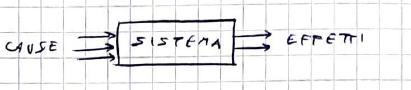
\includegraphics[width=0.75\linewidth]{automatica_mod_1_tex_assets/qa_p03_fig1.png}\par
\end{center}

% Pagina originale 4
\pagina{4}
Idealmente $y(t)=k_c r(t)$ e $e(t)=0$ per ogni $t$. $k_c$ è la costante di proporzionalità, $e(t)$ il segnale dell'errore:
\[e(t):=k_c r(t)-y(t).\]
Se $e(t)=0$ il problema è risolto. Se il riferimento è costante (setpoint) si parla di problema di regolazione; se è variabile si parla di controllo.
\subsection*{Controllo ad anello aperto}
\[r(t)\longrightarrow\boxed{C}\xrightarrow{u(t)}\boxed{S}\xrightarrow{}y(t),\qquad r(t)\longrightarrow\boxed{S\circ C}\longrightarrow y(t).\]
$C$ è il controllore, $S$ il sistema, $S\circ C$ il sistema di controllo. L'anello aperto ha poco controllo del sistema. Viene dato un obiettivo e conoscendo la risposta iniziale possiamo risolvere il problema solo ed esclusivamente in assenza di disturbi.
\subsection*{Controllo ad anello chiuso}
Il riferimento $r$ attraversa il controllore $C$, quindi $u$ entra in $S$ e produce $y$. Il punto di prelievo sull'uscita alimenta il sensore $M$; la sua uscita $\widetilde y$ ritorna al nodo di confronto sul ramo di retroazione (azione).

\begin{center}
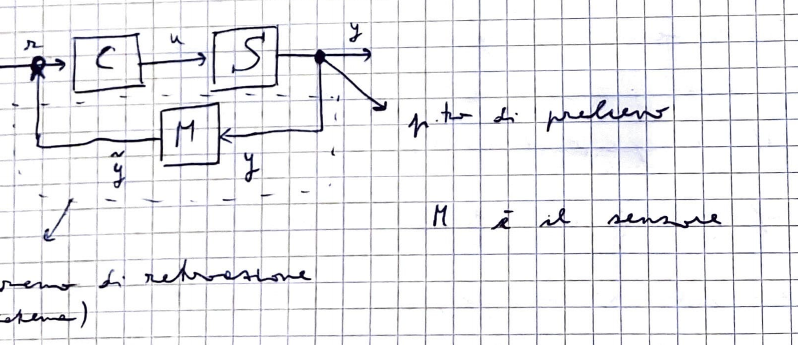
\includegraphics[width=0.75\linewidth]{automatica_mod_1_tex_assets/qa_p04_fig1.png}\par
\end{center}

% Pagina originale 5
\pagina{5}
\subsection*{Retroazione}
Un sistema ad anello chiuso può essere a retroazione negativa (positiva) se interrompendo l'anello in qualsiasi punto e inserendo una perturbazione a valle dell'interruzione, questa ritorna a monte dell'interruzione con segno contrario (stesso segno).
\paragraph{Esempio: retroazione negativa.}
$T=26\,^{\circ}\mathrm C$, $\overline T=25\,^{\circ}\mathrm C$, $e=1\,^{\circ}\mathrm C\Rightarrow u=-1\,^{\circ}\mathrm C$: abbassa di 1.
$T=24\,^{\circ}\mathrm C$, $\overline T=25\,^{\circ}\mathrm C$, $e=-1\,^{\circ}\mathrm C\Rightarrow u=1\,^{\circ}\mathrm C$: alza di 1. Questa è la retroazione negativa dove $u=-e$.
\paragraph{Esempio: retroazione positiva.}
$T=26\,^{\circ}\mathrm C$, $\overline T=25\,^{\circ}\mathrm C$, $e=1\,^{\circ}\mathrm C\Rightarrow u=1\,^{\circ}\mathrm C$: alza di 1.
$T=24\,^{\circ}\mathrm C$, $\overline T=25\,^{\circ}\mathrm C$, $e=-1\,^{\circ}\mathrm C\Rightarrow u=-1\,^{\circ}\mathrm C$: abbassa di 1. Questa è la retroazione positiva dove $u=e$.
Il grafico mostra la ricerca del setpoint $\bar r(t)$, un nuovo disturbo all'istante $\bar t$, l'effetto di disturbi misurabili e l'effetto di disturbi compensati. Non sarebbe possibile senza l'anello chiuso.
La retroazione è insita ovunque. Basta avere un sensore per avere retroazione (è un fatto che venga progettata).

\begin{center}
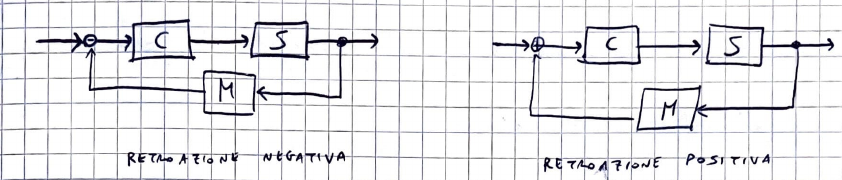
\includegraphics[width=0.75\linewidth]{automatica_mod_1_tex_assets/qa_p05_fig1.png}\par
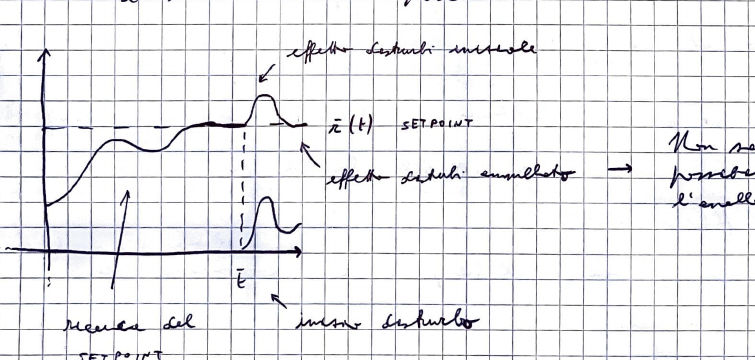
\includegraphics[width=0.75\linewidth]{automatica_mod_1_tex_assets/qa_p05_fig2.png}\par
\end{center}

% Pagina originale 6
\pagina{6}
\subsection*{Schema a blocchi di un sistema di controllo}
\[r(t)\to\boxed{\text{filtro ingresso}}\to\hat r(t)\to\oplus\xrightarrow{e(t)}\boxed C\xrightarrow{u(t)}\boxed A\to\boxed S\to y(t).\]
L'uscita ritorna tramite $M$ al nodo sommatore con segno negativo, come $\hat y(t)$. Il disturbo $d_A$ entra nell'attuatore $A$, $d_S$ nel sistema $S$, e $n(t)$ nel sensore $M$.
$\oplus$ è il nodo sommatore. $\hat y(t)$ è la stima dell'uscita (quella misurata tramite sensori); $\hat r(t)$ è il riferimento scalato; $d_A$ è il disturbo che agisce nell'attuatore; $d_S$ quello che agisce nel sistema; $n(t)$ è il disturbo sulla misura, ``rumore'' (noise).
\[\text{Attuatore}+\text{Sistema}=\text{Impianto (plant)}.\]
\subsection*{Tassonomia dei sistemi}
Statico se la sua uscita al tempo $\bar t$ dipende solo dall'ingresso al tempo $\bar t$. Dinamico se non è statico. Sono dinamici i sistemi modellabili tramite relazioni integro-differenziali. Per conoscere l'uscita al tempo $\bar t$ devi conoscere le condizioni iniziali.
Causali se l'uscita al tempo $\bar t$ non dipende dai valori futuri dell'ingresso (c'è un nesso di causa-effetto). Non causali se non sono causali.

\begin{center}
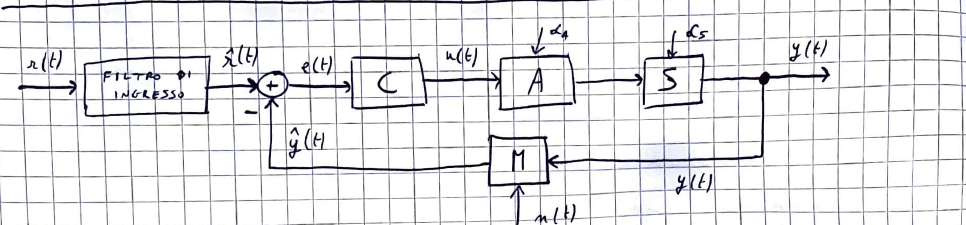
\includegraphics[width=0.75\linewidth]{automatica_mod_1_tex_assets/qa_p06_fig1.png}\par
\end{center}

% Pagina originale 7
\pagina{7}
Tempo invarianti se e solo se l'uscita prodotta dal sistema in risposta a un ingresso $\bar u$ ritardato di $\tau>0$ secondi è pari all'uscita senza ritardo dell'ingresso $\bar u$. Indica che il sistema non dipende dal momento in cui viene utilizzato e/o dalle condizioni o eventi precedenti.
Tempo variante se non è tempo invariante. Lineare se vale il PSE; non lineare se non vale il PSE. Tempo continuo se $t$ varia con continuità ($t\in\mathbb R$); tempo discreto se $t$ varia in un insieme con relazione $\bar t=kt_0$, $k\in\mathbb N$ ($t_0$ tempo di campionamento).
\subsection*{Principio di sovrapposizione degli effetti (PSE)}
Applico separatamente $u_i(t)$ ingressi e produco $y_i(t)$ uscite. Date $m$ costanti $k_i$, applicando
\[u(t)=\sum_{i=1}^{m}k_i u_i(t),\qquad y(t)=\sum_{i=1}^{m}k_i y_i(t).\]
Vale solo per sistemi lineari.
\subsection*{Risposte libera e forzata}
La soluzione di un'equazione differenziale $y(t)$ si può scrivere in due contributi:
\[y(t)=y_l(t)+y_f(t).\]
$y_l(t)$ è la risposta libera ($u(t)=0$); $y_f(t)$ è la risposta forzata (condizioni iniziali nulle); $y$ è la risposta completa.
% Pagina originale 8
\pagina{8}
\subsection*{Segnale causale e segnali canonici}
È causale se $x(t)=0$ per ogni $t<0$.
Impulso di durata finita:
\[P_\tau(t)=\begin{cases}1/\tau&0\le t\le\tau,\\0&\text{altrove},\end{cases}\qquad \int_{-\infty}^{\infty}P_\tau(t)\,dt=1.\]
Delta di Dirac: $\delta(t)\triangleq\lim_{\tau\to0}P_\tau(t)$; rappresentazione intuitiva $\delta(t)=\infty$ per $t=0$, $0$ per $t\ne0$. Proprietà:
\[\forall\varepsilon>0:\ \int_{-\varepsilon}^{\varepsilon}\delta(t)\,dt=1\quad(\text{massa}),\qquad \int_{-\infty}^{\infty}\delta(t-\tau)f(t)\,dt=f(\tau)\quad(\text{campionamento}).\]
Dimostrazione: $\delta(t-\tau)f(t)=\delta(t-\tau)f(\tau)$; quindi l'integrale è $f(\tau)\int_{-\infty}^{\infty}\delta(t-\tau)dt=f(\tau)$.
Gradino unitario:
\[1(t)=\begin{cases}1&t\ge0,\\0&t<0.\end{cases}\]
Qualsiasi ingresso costante a tratti può essere espresso come combinazione lineare di segnali a gradino opportunamente ritardati nel tempo.

\begin{center}
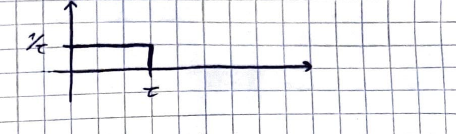
\includegraphics[width=0.75\linewidth]{automatica_mod_1_tex_assets/qa_p08_fig1.png}\par
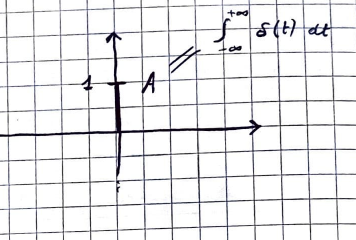
\includegraphics[width=0.75\linewidth]{automatica_mod_1_tex_assets/qa_p08_fig2.png}\par
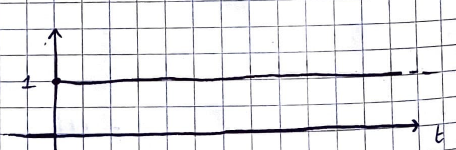
\includegraphics[width=0.75\linewidth]{automatica_mod_1_tex_assets/qa_p08_fig3.png}\par
\end{center}

% Pagina originale 9
\pagina{9}
\[P_\tau(t)=\frac1\tau1(t)-\frac1\tau1(t-\tau).\]
Rampa unitaria: $f(t)=t$ per $t\ge0$, $0$ per $t<0$, ossia $f(t)=t1(t)$. Rampa parabolica: $f(t)=t^2/2$ per $t\ge0$, $0$ per $t<0$, ossia $f(t)=\frac{t^2}{2}1(t)$.
\subsection*{Relazioni tra segnali canonici}
\[\delta\xrightarrow{\int}1(t)\xrightarrow{\int}t1(t)\xrightarrow{\int}\frac{t^2}{2}1(t).\]
Per $\bar t>0$:
\[\int_{-\infty}^{\bar t}\delta(t)dt=\int_{-\infty}^{0^-}\delta(t)dt+\int_{0^-}^{0^+}\delta(t)dt+\int_{0^+}^{\bar t}\delta(t)dt=1.\]
Per $\bar t<0$ l'integrale è zero. Dunque
\[\int_{-\infty}^{\bar t}\delta(t)dt=1(\bar t),\quad\int_{-\infty}^{\bar t}1(t)dt=\bar t1(\bar t),\quad\int_{-\infty}^{\bar t}t1(t)dt=\frac{\bar t^2}{2}1(\bar t).\]
\[\frac d{dt}\left[\frac{t^2}2 1(t)\right]=t1(t),\qquad\frac d{dt}[t1(t)]=1(t),\qquad\frac d{dt}1(t)\triangleq\delta(t).\]
La derivata generalizzata di $1(t)$ è $\delta(t)$.

\begin{center}
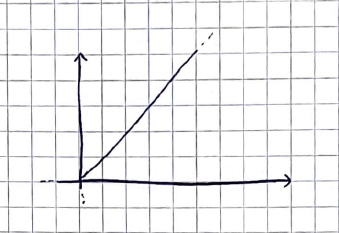
\includegraphics[width=0.75\linewidth]{automatica_mod_1_tex_assets/qa_p09_fig1.png}\par
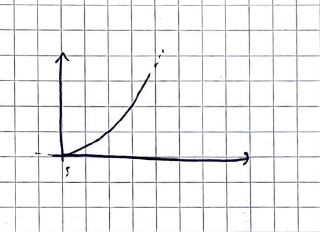
\includegraphics[width=0.75\linewidth]{automatica_mod_1_tex_assets/qa_p09_fig2.png}\par
\end{center}

\[\frac{d}{dt}\left[\frac{t^2}{2}1(t)\right]=
\begin{cases}\frac{d}{dt}\frac{t^2}{2}&t\ge0,\\\frac{d}{dt}0&t<0\end{cases}
=\begin{cases}t&t\ge0,\\0&t<0\end{cases}=t1(t).\]

% Pagina originale 10
\pagina{10}
\subsection*{Risposta all'impulso}
$g(t)$ è la risposta forzata di un sistema LTI a $\delta(t)$; è chiamata risposta all'impulso.
\subsection*{Integrale di convoluzione}
Approssimo $u(t)$ con un segnale costante a tratti espresso come somma di impulsi:
\begin{align*}
u(t)&\simeq\sum_i P_{\Delta\tau}(t-\tau_i)u(\tau_i)\Delta\tau\\
&=\sum_i\begin{cases}\frac1{\Delta\tau}u(\tau_i)\Delta\tau&t\in[\tau_i,\tau_{i+1}],\\0&\text{altrove}\end{cases}\\
&=\sum_{i=0}^{m-1}u(\tau_i)[1(t-\tau_i)-1(t-\tau_{i+1})].
\end{align*}
Se $\Delta\tau\to0$, la differenza dei gradini tende a $\delta(t-\tau_i)\Delta\tau$. Se $g(t)$ è la risposta a $\delta(t)$, allora $\Delta\tau g(t-\tau_i)$ è la risposta a $\Delta\tau\delta(t-\tau_i)$. Per il PSE:
\[y_f(t)\simeq\sum_{i=0}^{m-1}g(t-\tau_i)u(\tau_i)\Delta\tau.\]
Visto che $\Delta\tau\to0\Rightarrow m\to\infty$, la somma diventa un integrale:
\[y_f(t)=\int_0^\infty u(\tau)g(t-\tau)d\tau=u(t)*g(t)=g(t)*u(t).\]
L'asterisco è l'operatore convoluzione. Separando l'integrale a $t$, la parte da $t$ a $\infty$ è nulla poiché $g(x)=0$ per $x<0$.

\begin{center}
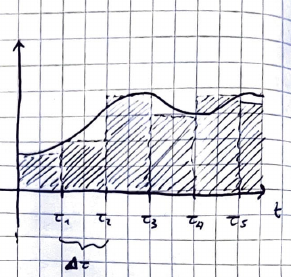
\includegraphics[width=0.75\linewidth]{automatica_mod_1_tex_assets/qa_p10_fig1.png}\par
\end{center}

\[u(t)=\sum_{i=0}^{m-1}u(\tau_i)[1(t-\tau_i)-1(t-\tau_{i+1})]
\xrightarrow{\Delta\tau\to0}\sum_{i=0}^{m-1}u(\tau_i)\delta(t-\tau_i)\Delta\tau.\]
\[y_f(t)=\int_0^t u(\tau)g(t-\tau)d\tau+
\underbrace{\int_t^\infty u(\tau)g(t-\tau)d\tau}_{0:\ g(x)=0\text{ per }x<0}.\]
\emph{Nota di trascrizione (p.~10): nella riga manoscritta con $1/\Delta\tau$ il membro destro contiene anche $\Delta\tau$; la riga successiva mostra la decomposizione degli impulsi. Si conserva qui la decomposizione leggibile.}

% Pagina originale 11
\pagina{11}
La convoluzione corrisponde al prodotto tra segnali:
\[y_f(t)=\int_0^t u(\tau)g(t-\tau)d\tau.\]
Il disegno rappresenta lo scorrimento del segnale $g(t-\tau)$ rispetto a $u(\tau)$ e l'area del loro prodotto.
\subsection*{Trasformata di Laplace}
L'operatore ``trasformata unilaterale di Laplace'' è una trasformazione che associa ad una funzione causale $f:\mathbb R\to\mathbb R$ una funzione $F(s):\mathbb C\to\mathbb C$:
\[\mathcal L\{f(t)\}=F(s)\triangleq\int_{0^-}^{\infty}e^{-st}f(t)dt,\qquad s=\sigma+j\omega.\]
Si richiede $e^{-st}\to0$ quando $t\to\infty$.
\[\mathcal L\{\delta(t)\}=\int_{0^-}^{\infty}e^{-st}\delta(t)dt=e^{-s0}=1\]
sfruttando la proprietà del campionamento. $\mathcal L\{\delta(t)\}=\Delta(s)=1$.
\[\mathcal L\{1(t)\}=\int_0^\infty e^{-st}dt=-\frac1s[e^{-st}]_0^\infty=-\frac1s(0-1)=\frac1s\]
solo se $\operatorname{Re}s>0$. Infatti $|e^{-st}|=|e^{-\sigma t}||e^{-j\omega t}|=|e^{-\sigma t}|$, il cui limite è $0$ se $\sigma>0$, $1$ se $\sigma=0$, $\infty$ se $\sigma<0$.

\begin{center}
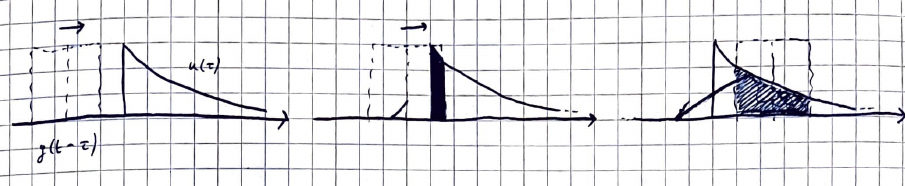
\includegraphics[width=0.75\linewidth]{automatica_mod_1_tex_assets/qa_p11_fig1.png}\par
\end{center}

% Pagina originale 12
\pagina{12}
\subsection*{Proprietà della trasformata}
\begin{enumerate}
\item Linearità:
\[\mathcal L\{\alpha f_1(t)+\beta f_2(t)\}=\alpha\mathcal L\{f_1(t)\}+\beta\mathcal L\{f_2(t)\}.\]
Dimostrazione: dalla linearità dell'integrale.
\item $\mathcal L\{f(t-\tau)\}=e^{-s\tau}\mathcal L\{f(t)\}$. Ponendo $T=t-\tau$:
\[\int_{0^-}^\infty f(t-\tau)e^{-st}dt=\int_{0^- -\tau}^{\infty}f(T)e^{-s(T+\tau)}dT=e^{-s\tau}\int_0^\infty f(T)e^{-sT}dT.\]
\item $\mathcal L\{f(t)e^{at}\}=F(s-a)$. Infatti $\int_{0^-}^{\infty}f(t)e^{at}e^{-st}dt=\int_{0^-}^{\infty}f(t)e^{-(s-a)t}dt$.
\item $\mathcal L\{t^m f(t)\}=(-1)^m\frac{d^mF(s)}{ds^m}$. Per $m=1$:
\[\frac d{ds}F(s)=\int_{0^-}^{\infty}\frac d{ds}e^{-st}f(t)dt=\int_{0^-}^{\infty}(-t)e^{-st}f(t)dt=-\mathcal L\{tf(t)\}.\]
Si continua per induzione.
\item $\mathcal L\{f^{(m)}(t)\}=s^mF(s)-s^{m-1}f(0)-\cdots-f^{(m-1)}(0)$. Se le condizioni iniziali sono tutte nulle: $\mathcal L\{f^{(m)}(t)\}=s^mF(s)$.
\item $\mathcal L\{\int_0^t f(\tau)d\tau\}=\frac1sF(s)$.
\end{enumerate}
\paragraph{Passaggi della dimostrazione della proprietà 3.}
Ponendo $z=s-a$:
\[\int_{0^-}^{\infty}f(t)e^{-(s-a)t}dt
=\int_{0^-}^{\infty}f(t)e^{-zt}dt=F(z)=F(s-a).\]
\paragraph{Passaggi della proprietà 4.}
\[\frac d{ds}F(s)=\frac d{ds}\int_{0^-}^{\infty}e^{-st}f(t)dt
=\int_{0^-}^{\infty}\frac d{ds}(e^{-st})f(t)dt
=\int_{0^-}^{\infty}f(t)(-t)e^{-st}dt.\]

% Pagina originale 13
\pagina{13}
\subsection*{Esempi di trasformate}
\begin{align*}
\mathcal L\{e^{-at}1(t)\}&=\left.\frac1s\right|_{s+a}=\frac1{s+a},\\
\mathcal L\{t1(t)\}&=-\frac d{ds}\frac1s=\frac1{s^2},\\
\mathcal L\{\tfrac{t^2}2 1(t)\}&=\frac12\frac{d^2}{ds^2}\frac1s=\frac1{s^3},\\
\mathcal L\{\sin(\omega t)1(t)\}&=\frac1{2j}\left(\frac1{s-j\omega}-\frac1{s+j\omega}\right)=\frac\omega{s^2+\omega^2},\\
\mathcal L\{\cos(\omega t)1(t)\}&=\frac12\left(\frac1{s-j\omega}+\frac1{s+j\omega}\right)=\frac s{s^2+\omega^2}.
\end{align*}
Si usano $\sin(\omega t)=(e^{j\omega t}-e^{-j\omega t})/(2j)$ e $\cos(\omega t)=(e^{j\omega t}+e^{-j\omega t})/2$.
\subsection*{Teorema del valor finale}
Sia $f(t)$ un segnale causale al quale è associato $F(s)=\mathcal L\{f(t)\}$. Se esiste $\lim_{t\to\infty}f(t)\in\mathbb R$, allora
\[\lim_{t\to\infty}f(t)=\lim_{s\to0}sF(s),\]
e $sF(s)$ ha tutte le singolarità nel semipiano sinistro ($\operatorname{Re}s<0$). Le singolarità sono i valori di $s$ dove $sF(s)\to\infty$, cioè i poli.
\subsection*{Teorema del valor iniziale}
\[\lim_{t\to0}f(t)=\lim_{s\to\infty}sF(s).\]
\paragraph{Passaggi delle trasformate.}
\begin{align*}
\mathcal L\{t1(t)\}&=\frac d{ds}\frac1s(-1)^1=-\left(-\frac1{s^2}\right)=\frac1{s^2},\\
\mathcal L\{\tfrac{t^2}{2}1(t)\}&=\frac12\frac{d^2}{ds^2}\frac1s(-1)^2
=\frac12\frac d{ds}\left(-\frac1{s^2}\right)=\frac12\frac2{s^3}=\frac1{s^3},\\
\mathcal L\{\sin(\omega t)1(t)\}&=\mathcal L\{\tfrac{e^{j\omega t}-e^{-j\omega t}}{2j}1(t)\}\\
&=\tfrac1{2j}\mathcal L\{e^{j\omega t}1(t)\}-\tfrac1{2j}\mathcal L\{e^{-j\omega t}1(t)\}\\
&=\tfrac1{2j}\tfrac1{s-j\omega}-\tfrac1{2j}\tfrac1{s+j\omega}
=\tfrac1{2j}\tfrac{2j\omega}{s^2+\omega^2},\\
\mathcal L\{\cos(\omega t)1(t)\}&=\mathcal L\{\tfrac{e^{j\omega t}+e^{-j\omega t}}2 1(t)\}\\
&=\tfrac12\mathcal L\{e^{j\omega t}1(t)\}+\tfrac12\mathcal L\{e^{-j\omega t}1(t)\}
=\tfrac12\tfrac{2s}{s^2+\omega^2}.
\end{align*}

% Pagina originale 14
\pagina{14}
\subsection*{Trasformata della convoluzione}
\[h(t)=f_1(t)*f_2(t)=\int_{-\infty}^{\infty}f_1(t-\tau)f_2(\tau)d\tau=\int_{0^-}^{t}f_1(t-\tau)f_2(\tau)d\tau.\]
\[\mathcal L\{h(t)\}=\int_0^\infty\left[\int_0^t f_1(t-\tau)f_2(\tau)d\tau\right]e^{-st}dt=F_1(s)F_2(s).\]
Quindi $\mathcal L\{f_1*f_2\}=\mathcal L\{f_1\}\mathcal L\{f_2\}$. So che $y_f(t)=g(t)*u(t)$, perciò $Y_f(s)=G(s)U(s)$, rappresentato dal blocco $U(s)\to\boxed{G(s)}\to Y(s)$.
\subsection*{Trovare $G(s)$ senza conoscere $g(t)$}
1) $G(s)=Y_f(s)/U(s)$. 2) Conoscendo il modello matematico del sistema:
\[\sum_{i=0}^{n}a_iD^iy(t)=\sum_{i=0}^{m}b_iD^iu(t),\qquad n\ge m,\quad a_i,b_i\in\mathbb R.\]
Applico Laplace e la linearità:
\[\sum_{i=0}^{n}a_i\left(s^iY(s)-\sum_{j=0}^{i-1}y^{(i-j-1)}(0)s^j\right)=\sum_{i=0}^{m}b_i s^iU(s),\]
con condizioni iniziali dell'ingresso nulle. Riordinando:
\[\underbrace{\sum_{i=0}^{n}a_i s^i}_{a(s)}Y(s)-\underbrace{\sum_{i=0}^{n}\sum_{j=0}^{i-1}a_i y^{(i-j-1)}(0)s^j}_{c(s)}=\underbrace{\sum_{i=0}^{m}b_i s^i}_{b(s)}U(s).\]
$a(s)$ è di grado $n$, $c(s)$ di grado $n-1$, $b(s)$ di grado $m$.
\paragraph{Passaggio mediante la linearità.}
\[\mathcal L\left\{\sum_{i=0}^n a_iD^iy(t)\right\}
=\mathcal L\left\{\sum_{i=0}^m b_iD^iu(t)\right\}
\quad\Longrightarrow\quad
\sum_{i=0}^n a_i\mathcal L\{D^iy(t)\}
=\sum_{i=0}^m b_i\mathcal L\{D^iu(t)\}.\]
$n\ge m$: sistema causale.

% Pagina originale 15
\pagina{15}
\[a(s)Y(s)-c(s)=b(s)U(s)\Rightarrow Y(s)=\underbrace{\frac{b(s)}{a(s)}U(s)}_{Y_f(s)}+\underbrace{\frac{c(s)}{a(s)}}_{Y_l(s)}.\]
\[G(s)=\frac{b(s)}{a(s)}=\frac{b_ms^m+b_{m-1}s^{m-1}+\cdots+b_1s+b_0}{a_ns^n+a_{n-1}s^{n-1}+\cdots+a_1s+a_0}.\]
È la funzione di trasferimento. Esempio:
\[2\frac{d^3y}{dt^3}+3\frac{d^2y}{dt^2}+2\frac{dy}{dt}-y=3\frac{du}{dt}-5u,\qquad G(s)=\frac{3s-5}{2s^3+3s^2+2s-1}.\]
\subsection*{Proprietà FDT}
È una funzione razionale fratta; $G(s)=Y_f(s)/U(s)=b(s)/a(s)$; $G(s)=\mathcal L\{g(t)\}$, trasformata della risposta all'impulso.
Con $m=\deg b$, $n=\deg a$, può essere propria ($m=n$), strettamente propria ($m<n$), impropria ($m>n$, non causale quindi). Esempi: $(s^2+2s+2)/(s^2+3)$, $(s-1)/(s^4+2)$, $s^2/(s-1)$ rispettivamente.
\subsection*{Poli e zeri}
Poli: tutte le $n$ radici complesse di $a(s)$ dove $|G(s)|\to\infty$. Zeri: tutte le $m$ radici complesse di $b(s)$ dove $G(s)=0$.

\begin{center}
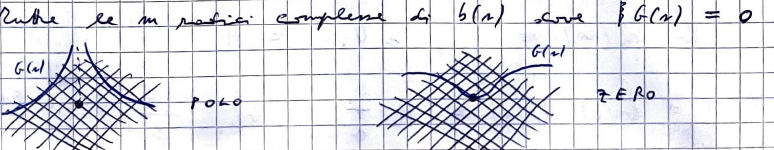
\includegraphics[width=0.75\linewidth]{automatica_mod_1_tex_assets/qa_p15_fig1.png}\par
\end{center}

% Pagina originale 16
\pagina{16}
\subsection*{Rappresentazione della FDT}
\[G(s)=\frac{\sum b_i s^i}{\sum a_i s^i}=\frac{b_m}{a_n}\frac{\prod(s-z_i)}{\prod(s-p_i)}=k_0\frac{\prod(s-z_i)}{\prod(s-p_i)},\quad k_0=\frac{b_m}{a_n}.\]
\subsection*{Mappa poli-zeri}
Per $G(s)=(s+3)/[(s-1)(s+1)(s+2)^2]$, zero in $-3$ (cerchio), poli in $-2$ (doppio), $-1$, $1$ (croci). Il grafico esprime $G(s)/k_0$ e non $G(s)$.
\[G(s)=k_0\frac{\prod(-z_i)\prod(1-s/z_i)}{\prod(-p_i)\prod(1-s/p_i)}=k_1\frac{\prod(1+\tau_{z_i}s)}{\prod(1+\tau_{p_i}s)},\]
\[k_1=k_0\frac{\prod(-z_i)}{\prod(-p_i)},\quad \tau_{z_i}=-\frac1{z_i},\quad\tau_{p_i}=-\frac1{p_i}.\]
$k_1$ è il guadagno statico del sistema; le $\tau$ sono costanti di tempo [s]. Osservo che $G(0)=k_1$.
Considero un ingresso a gradino $u(t)=M1(t)$, $U(s)=M/s$:
\[y(\infty)=\lim_{s\to0}sY(s)=\lim_{s\to0}sG(s)U(s)=\lim_{s\to0}MG(s)=Mk_1.\]
Calcolo $u(\infty)=\lim_{s\to0}sU(s)=M$.

\begin{center}
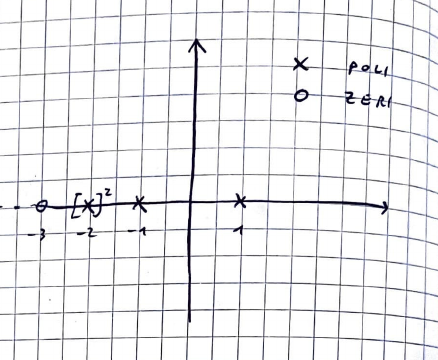
\includegraphics[width=0.75\linewidth]{automatica_mod_1_tex_assets/qa_p16_fig1.png}\par
\end{center}

\[G(0)=k_1\frac{\prod(1+\tau_{z_i}0)}{\prod(1+\tau_{p_i}0)}
=k_1\frac{\prod1}{\prod1}=k_1.\]
\emph{Nota di trascrizione (pp.~16--17): compaiono anche le scritture $Y(0)=G(0)U(0)$ e
\[G(0)=\frac{Y(0)}{U(0)}=\frac{s^{-1}y(\infty)}{s^{-1}u(\infty)}.\]
Per l'ingresso a gradino, $U(s)=M/s$ e $Y(s)$ non hanno in generale valori finiti in $s=0$; il rapporto a regime è quello ottenuto dal limite sopra.}

% Pagina originale 17
\pagina{17}
\[k_1=G(0)=\frac{y(\infty)}{u(\infty)}\qquad\text{guadagno statico}.\]
$k_1$ è il rapporto tra valore finale dell'uscita e valore finale dell'ingresso. Se $k_1>1$ l'uscita sarà amplificata ($y(\infty)>u(\infty)$); se $k_1\le1$ sarà attenuata ($y(\infty)\le u(\infty)$).
\subsection*{Velocità del sistema}
Più il polo è lontano dall'asse immaginario, più veloce sarà il sistema a portarsi a regime. Nel disegno $p_2<p_1<0$ e la risposta relativa a $p_2$ decade più rapidamente.
\subsection*{Antitrasformata di Laplace}
\[\mathcal L^{-1}\{F(s)\}=f(t)=\frac1{2\pi j}\int_{\sigma_0-j\infty}^{\sigma_0+j\infty}F(s)e^{st}ds.\]
$Y(s)=\frac ba U(s)+\frac ca$. Essendo $U(s)$ una funzione razionale fratta, $Y(s)$ sarà lo stesso:
\[\mathcal L^{-1}\{Y(s)\}=\mathcal L^{-1}\left\{\frac{N(s)}{D(s)}\right\},\qquad N,D\text{ polinomi in }s.\]
$Y(s)$ può essere propria o strettamente propria. Se propria:
\[Y(s)=q_0+\frac{R(s)}{D(s)}\Rightarrow y(t)=q_0\delta(t)+\mathcal L^{-1}\left\{\frac{R(s)}{D(s)}\right\},\quad\deg R<\deg D.\]

\begin{center}
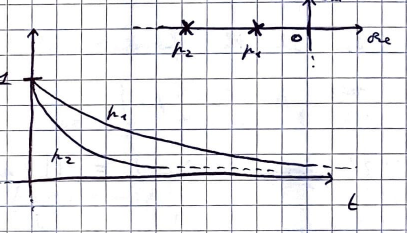
\includegraphics[width=0.75\linewidth]{automatica_mod_1_tex_assets/qa_p17_fig1.png}\par
\end{center}

% Pagina originale 18
\pagina{18}
Per $Y(s)$ strettamente propria rendo $D(s)$ monico raccogliendo il coefficiente del termine di grado massimo: $D(s)=s^\ell+d_{\ell-1}s^{\ell-1}+\cdots+d_0$.
Primo caso: radici tutte distinte:
\[D(s)=\prod_i(s-p_i),\quad F(s)=\frac{N(s)}{D(s)}=\sum_{i=1}^{\ell}\frac{k_i}{s-p_i},\quad k_i\in\mathbb C.\]
\[\mathcal L^{-1}\{F(s)\}=\left[\sum_{i=1}^{\ell}k_i e^{p_it}\right]1(t).\]
Per il teorema fondamentale dell'algebra se $p_i\in\mathbb C$ anche il suo coniugato è tra le radici.
Secondo caso: radici multiple, $D(s)=\prod_i(s-p_i)^{\nu_i}$ con $\sum_i\nu_i=\ell$. Per ciascun termine:
\[\mathcal L^{-1}\left\{\frac{k}{(s-p_i)^\nu}\right\}=k\frac{t^{\nu-1}}{(\nu-1)!}e^{p_it}1(t).\]
\subsection*{Calcolo di $k_i$}
\[F(s)=\frac{N(s)}{\prod(s-p_i)}=\frac{k_1}{s-p_1}+\frac{k_2}{s-p_2}+\cdots+\frac{k_\ell}{s-p_\ell}.\]
Moltiplicando per $s-p_1$ e valutando in $s=p_1$ gli altri termini si annullano:
\[k_i=\left[(s-p_i)F(s)\right]_{s=p_i}.\]
\begin{align*}
(s-p_1)F(s)&=(s-p_1)\frac{k_1}{s-p_1}
 +(s-p_1)\frac{k_2}{s-p_2}+\cdots,\\
\left[(s-p_1)F(s)\right]_{s=p_1}
&=k_1+\left[(s-p_1)\frac{k_2}{s-p_2}\right]_{s=p_1}+\cdots=k_1.
\end{align*}
\emph{Nota di trascrizione (p.~18): lo sviluppo manoscritto del caso multiplo mostra un solo termine per polo; lo sviluppo completo, con tutte le potenze, è esplicitato alla p.~19. La proprietà dei coniugati presuppone coefficienti reali.}

\[F(s)=\frac{N(s)}{\prod_i(s-p_i)^{\nu_i}}
=\sum_{i=1}^j\frac{k_i}{(s-p_i)^{\nu_i}},\qquad
\mathcal L^{-1}\{F(s)\}=\left[\sum_{i=1}^j k_i\frac{t^{\nu_i-1}}{(\nu_i-1)!}e^{p_it}\right]1(t).\]
\emph{La riga precedente riproduce la forma abbreviata del manoscritto (p.~18); in generale, per ciascun polo multiplo occorrono anche tutte le potenze inferiori, come nella p.~19.}
% Pagina originale 19
\pagina{19}
\subsection*{Caso di poli complessi coniugati}
\[F(s)=\frac{N(s)}{\widetilde D(s)[(s-\sigma)^2+\omega^2]}=\frac{k_1}{s-\sigma-j\omega}+\frac{k_2}{s-\sigma+j\omega}+\sum_i\frac{k_i}{s-p_i}.\]
$k_1=\overline{k_2}$ perché $p_1=\overline{p_2}$. Scrivendo $k_1=u+jv$:
\begin{align*}
\mathcal L^{-1}\left\{\frac{k_1}{s-\sigma-j\omega}+\frac{k_2}{s-\sigma+j\omega}\right\}
&=[(u+jv)e^{(\sigma+j\omega)t}+(u-jv)e^{(\sigma-j\omega)t}]1(t)\\
&=e^{\sigma t}[u(e^{j\omega t}+e^{-j\omega t})+jv(e^{j\omega t}-e^{-j\omega t})]1(t)\\
&=2e^{\sigma t}(u\cos\omega t-v\sin\omega t)1(t).
\end{align*}
Dimostro che $A\cos\omega t+B\sin\omega t=R\cos(\omega t-\varphi)$. Poiché $\cos(\omega t-\varphi)=\cos\omega t\cos\varphi+\sin\omega t\sin\varphi$, segue $A=R\cos\varphi$, $B=R\sin\varphi$, $R=\sqrt{A^2+B^2}$ e $\tan\varphi=B/A$.
\[A\cos\omega t+B\sin\omega t=\sqrt{A^2+B^2}\cos(\omega t-\arctan(B/A)).\]
Pertanto il contributo coniugato è $2e^{\sigma t}|k|\cos(\omega t+\varphi_k)1(t)$.
\subsection*{Poli con molteplicità maggiore di uno}
\[F(s)=\frac{k_{i1}}{(s-p_i)^{\nu_i}}+\frac{k_{i2}}{(s-p_i)^{\nu_i-1}}+\cdots+\frac{k_{i\nu_i}}{s-p_i}+\cdots.\]
\[[(s-p_i)^{\nu_i}F(s)]_{s=p_i}=k_{i1},\qquad \frac d{ds}[(s-p_i)^{\nu_i}F(s)]=k_{i2}+2(s-p_i)k_{i3}+\cdots.\]
\paragraph{Passaggi intermedi.}
\[u e^{\sigma t}(e^{j\omega t}+e^{-j\omega t})
+jv e^{\sigma t}(e^{j\omega t}-e^{-j\omega t})
=2u e^{\sigma t}\cos(\omega t)-2v e^{\sigma t}\sin(\omega t).\]
\emph{Nota di trascrizione (p.~19): nella riga intermedia originale compare $2j^2v$; si usa $j^2=-1$. L'espressione della fase con $\arctan(B/A)$ riportata nel manoscritto richiede la scelta del quadrante appropriato.}
\[\begin{cases}A=R\cos\varphi,\\B=R\sin\varphi\end{cases}
\Longrightarrow\quad
\begin{cases}R=\sqrt{A^2+B^2},\\B/A=\tan\varphi\end{cases}
\Longrightarrow\quad
\begin{cases}R=\sqrt{A^2+B^2},\\\varphi=\arctan(B/A).\end{cases}\]
\[\left.\frac d{ds}\{F(s)(s-p_i)^{\nu_i}\}\right|_{s=p_i}
=k_{i2}+0+\cdots+0=k_{i2}.\]
% Pagina originale 20
\pagina{20}
Valutando la derivata in $s=p_i$ si ottiene $k_{i2}$. In generale:
\[k_{ij}=\frac1{(j-1)!}\left[\frac{d^{j-1}}{ds^{j-1}}\{F(s)(s-p_i)^{\nu_i}\}\right]_{s=p_i}.\]
\subsection*{Calcolare la risposta forzata a $\delta(t)$ conoscendo $G(s)$}
$y(t)=\frac d{dt}y_1(t)$, dove $y(t)$ è risposta all'impulso $\delta(t)$ e $y_1(t)$ risposta al gradino $1(t)$. Per linearità la risposta all'impulso è la derivata della risposta al gradino.
\[Y(s)=G(s)U(s)=G(s)\mathcal L\{\delta(t)\}=G(s).\]
\subsection*{Teorema dei residui}
\[\sum_{i=1}^{\ell}k_i=\begin{cases}0&n-m>1,\\b_m/a_n&n-m=1.\end{cases}\qquad y(0)=\sum_{i=1}^{\ell}k_i.\]
Per poli multipli si intende $k_i\triangleq k_{i\nu_i}$. Esempio:
\[\frac{k_1}{s-p_1}+\frac{k_2}{s-p_2}+\frac{k_{31}}{(s-p_3)^3}+\frac{k_{32}}{(s-p_3)^2}+\frac{k_{33}}{s-p_3},\qquad k_1+k_2+k_{33}=0.\]

\begin{center}
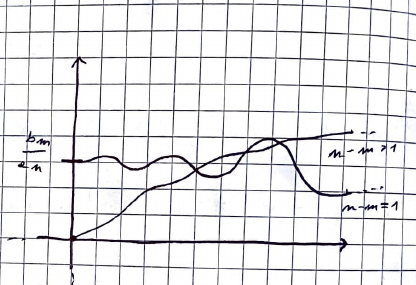
\includegraphics[width=0.75\linewidth]{automatica_mod_1_tex_assets/qa_p20_fig1.png}\par
\end{center}

% Pagina originale 21
\pagina{21}
\subsection*{Schema a blocchi}
Nodo sommatore: $E(s)=R(s)-Y(s)H(s)$.
Blocchi in serie: $G(s)=G_1(s)G_2(s)$.
Blocchi in parallelo: $U=U_1=U_2$, $Y=Y_1+Y_2=U_1G_1+U_2G_2=U(G_1+G_2)$; $G_{\rm eq}(s)=\sum_i G_i(s)$.
Retroazione:
\begin{align*}
Y(s)&=E(s)G(s)=[R(s)-X(s)]G(s)=[R(s)-Y(s)H(s)]G(s),\\
Y(s)+Y(s)H(s)G(s)&=R(s)G(s),\\
Y(s)[1+H(s)G(s)]&=R(s)G(s),\\
Y(s)&=R(s)\frac{G(s)}{1+H(s)G(s)}=R(s)G_{\rm eq}(s),\\
G_{\rm eq}(s)&=\frac{G(s)}{1\pm H(s)G(s)}.
\end{align*}
Il segno $+$ corrisponde alla retroazione negativa, il segno $-$ a quella positiva. $G$ è la FDT nel ramo diretto, $H$ nel ramo di retroazione.

\begin{center}
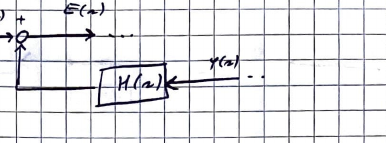
\includegraphics[width=0.75\linewidth]{automatica_mod_1_tex_assets/qa_p21_fig1.png}\par
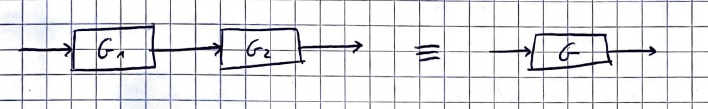
\includegraphics[width=0.75\linewidth]{automatica_mod_1_tex_assets/qa_p21_fig2.png}\par
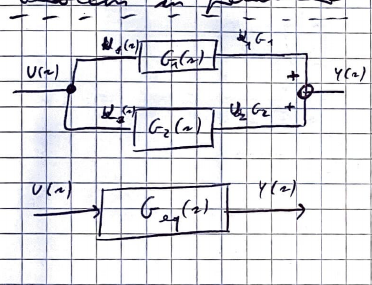
\includegraphics[width=0.75\linewidth]{automatica_mod_1_tex_assets/qa_p21_fig3.png}\par
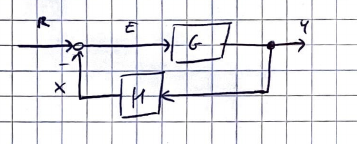
\includegraphics[width=0.75\linewidth]{automatica_mod_1_tex_assets/qa_p21_fig4.png}\par
\end{center}

% Pagina originale 22
\pagina{22}
\subsection*{Spostamento di punti di prelievo}
Un prelievo dopo $G$ si sposta prima di $G$ inserendo $G$ sul ramo prelevato. Un prelievo prima di $G$ si sposta dopo $G$ inserendo $1/G$ sul ramo prelevato.
\subsection*{Spostamento di nodi sommatori}
\[G(U+W)=GU+GW,\qquad GU+W=G(U+W/G).\]
Il nodo prima di $G$ si sposta dopo $G$ inserendo $G$ sul ramo secondario; quello dopo $G$ si sposta prima inserendo $1/G$.
\subsection*{Scambio di nodi sommatori}
Due sommatori consecutivi con ingressi $A$ e $B$ si possono scambiare. Se sono separati da $G$, spostando il secondo prima del blocco occorre inserire $1/G$ sul ramo $B$:
\[G(U+A)+B=G(U+A+B/G).\]

\begin{center}
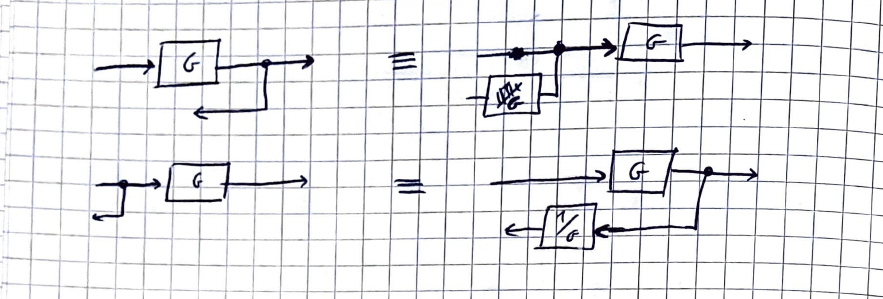
\includegraphics[width=0.86\linewidth]{automatica_mod_1_tex_assets/qa_p22_fig1.png}\par
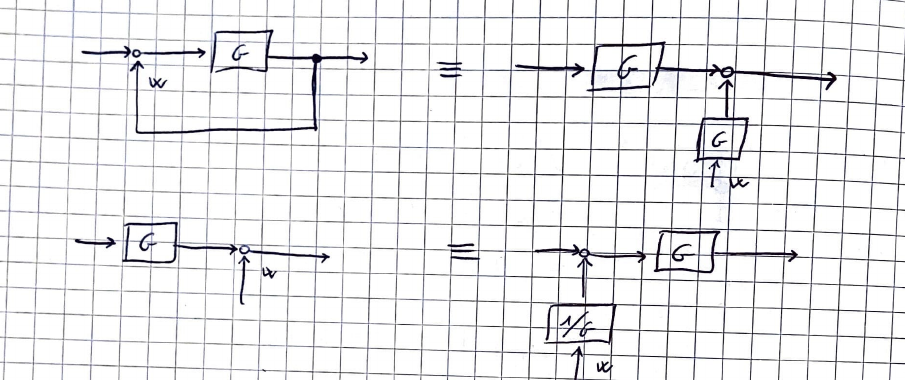
\includegraphics[width=0.86\linewidth]{automatica_mod_1_tex_assets/qa_p22_fig2.png}\par
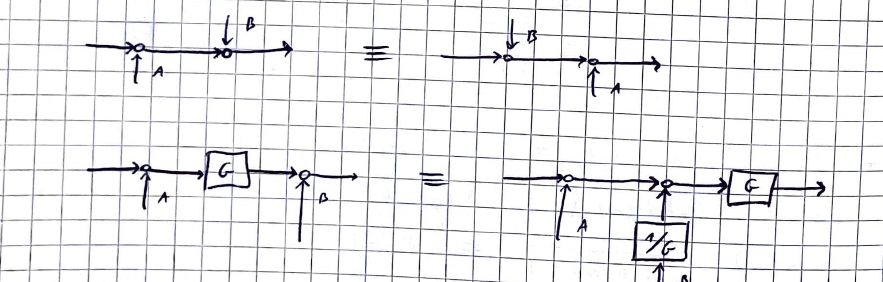
\includegraphics[width=0.86\linewidth]{automatica_mod_1_tex_assets/qa_p22_fig3.png}\par
\end{center}
